\normalfalse \difficiletrue \tdifficilefalse
\correctiontrue
%\UPSTIidClasse{11} % 11 sup, 12 spé
%\newcommand{\UPSTIidClasse}{11}

\exer{Banc hydraulique $\star$ \label{C2:03:stab:63}}
%% CCP MP 2010
\setcounter{numques}{0}
\UPSTIcompetence[2]{C2-03}
\index{Compétence C2-03}
\index{Schéma-blocs}
\index{Précision}

\ifcorrection
\else
\textbf{Pas de corrigé pour cet exercice.}
\fi

\ifprof
\else

Pour limiter l’erreur statique due aux fuites, on envisage d’asservir la pression d’eau dans le tube. 
%L’objectif est ici de proposer un réglage du correcteur pour répondre aux critères du cahier des charges.
La pression d’eau à l’intérieur du tube est mesurée par un capteur de pression. 

\begin{center}
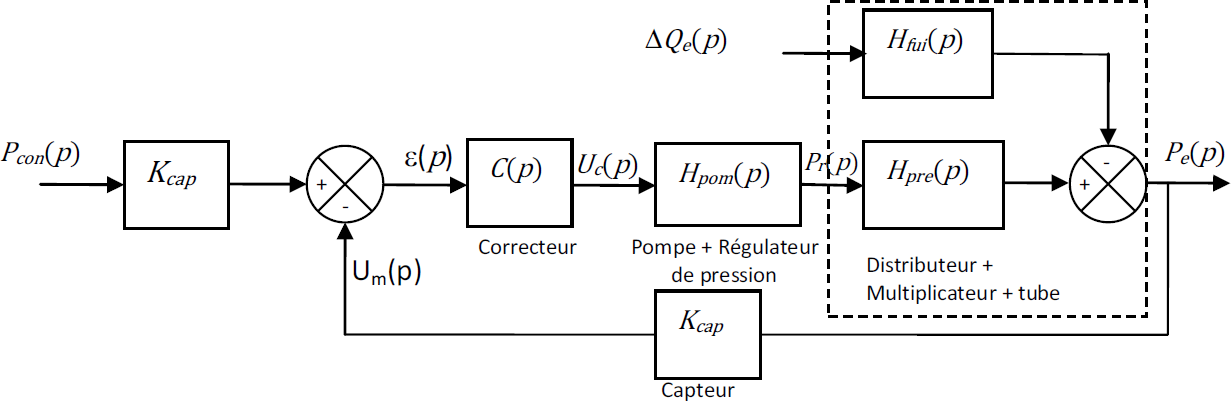
\includegraphics[width=\linewidth]{63_01}
\end{center}

 
 \begin{tabular}{lp{5cm}}
$P_{\text{con}}(p)$ : & 	pression de consigne d’eau dans le tube (Pa) \\
$P_e(p)$ : & 	pression d’eau dans le tube (Pa) \\
$U_c(p)$ : & 	tension de commande du régulateur de pression (V)\\
$P_r(p)$ : &	pression d’huile régulée (Pa)\\
$\Delta Q_e(p)$ :& 	débit de fuite (\si{m^3s^{-1}})\\
$U_m(p)$ 	:&	tension de mesure du capteur (V)\\
\end{tabular}
 
\textbf{ Hypothèses}
\begin{itemize}
\item L’ensemble de mise sous pression {tube + distributeur + multiplicateur de pression} est défini par les transmittances suivantes : $H_{\text{pre}} (p)=\dfrac{K_m}{1+T_1 p}$	et	$H_{\text{fui}} (p)=\dfrac{K_f}{1+T_1 p}$ avec 	$K_m = 3,24$ ; 	$K_f = \SI{2,55e10}{Pa.m^{-3}.s}$ ; 	$T_1  = \SI{10}{s}$.
\item L’ensemble {pompe+régulateur de pression} est modélisé par la fonction de transfert :
$H_{\text{pom}} (p)=\dfrac{K_{\text{pom}}}{1+T_2 p}$  avec 	$K_{\text{pom}} = \SI{1,234e7}{Pa/V}$; 	$T_2 = \SI{5}{s}$.
\item Le capteur est modélisé par un gain pur :	$K_{\text{cap}} = \SI{2,5e-8}{V/Pa}$.
\end{itemize}
La pression de consigne est de $P_{\text{con}} = \SI{800}{bars}$ et les débits de fuite sont estimés à $\Delta Q_e = \SI{5e-4}{m3/s}$.

 
Le cahier des charges concernant le réglage de la pression de test est le suivant.
\begin{center}
\begin{tabular}{lp{5cm}}
\hline 
Stabilité :  & marge de phase de 60\degres  \\
  	  &  marge de gain de \SI{12}{dB} \\ \hline
Rapidité :  &  temps d’établissement $t_e < \SI{40}{s}$ (voir remarque ci-dessous) \\ \hline
Précision : & 	erreur statique < 5\% soit pour une consigne de 800 bars : \\
&erreur statique due à la consigne : $\varepsilon_{\text{con}}< 5\%$  \\
& erreur statique due à la perturbation $\varepsilon_{\text{pert}} < \SI{40}{bars}$ \\ \hline
Amortissement :&	pas de dépassement \\ \hline
\end{tabular}
\end{center}

Dans le cas d’un système bouclé convenablement amorti, on pourra utiliser, sans aucune justification, la relation :
$t_e \cdot \omega_{\SI{0}{dB}}=3$ où $\omega_{\SI{0}{dB}}$ désigne la pulsation de coupure à \SI{0}{dB} en boucle ouverte et $t_e$ le temps d’établissement en boucle fermée vis-à-vis d’un échelon de consigne :
\begin{itemize}
\item $t_e = t_m$, temps du 1er maximum si le dépassement est supérieur à \SI{5}{\%},
\item $t_e = t_R$, temps de réponse à \SI{5}{\%} si le dépassement est nul ou inférieur à \SI{5}{\%}.
\end{itemize}

On se propose de corriger le système avec le correcteur défini sur le schéma bloc ci-dessous.

\begin{center}
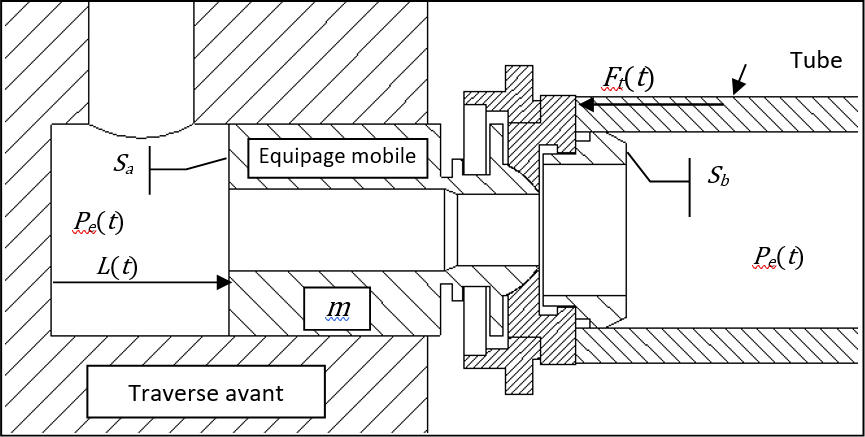
\includegraphics[width=5cm]{63_02}
\end{center}
\fi

\question{Déterminer la fonction de transfert $C(p)$ de ce correcteur.}
\ifprof
On a $C(p)=\dfrac{K_i}{p}+K_p = \dfrac{K_i+p K_p}{p} = K_i \dfrac{1+p \dfrac{K_p}{K_i}}{p}$.
\else 
\fi


\question{Tracer l’allure de son diagramme de Bode en fonction des coefficients $K_i$ et $K_p$.}
\ifprof

\begin{center}
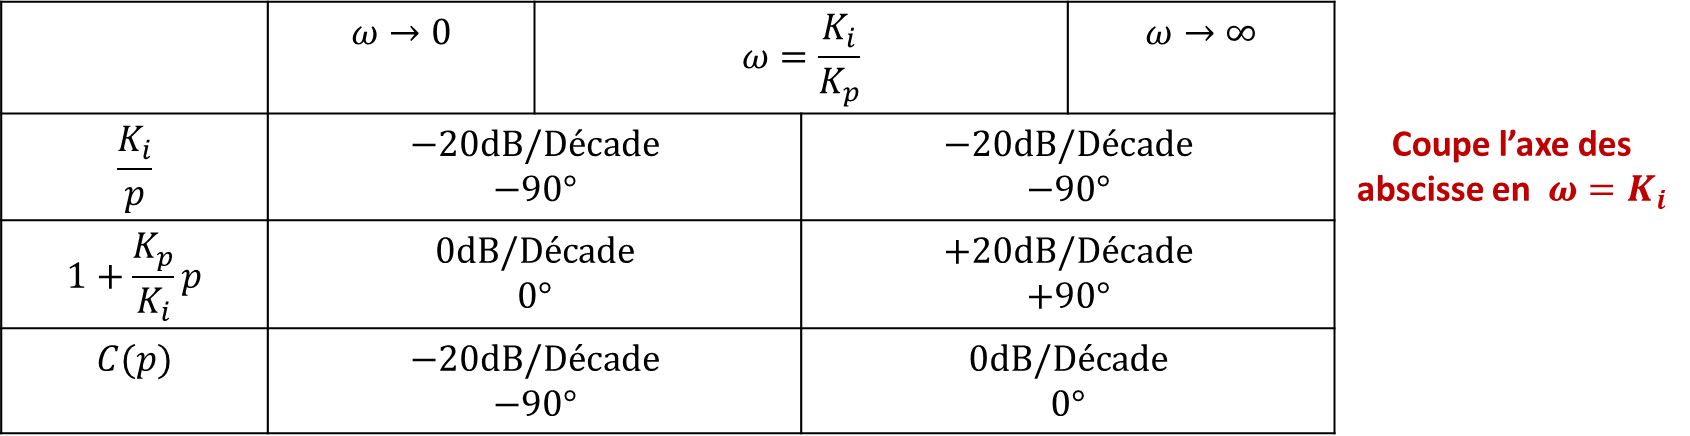
\includegraphics[width=12cm]{63_02_cor}
\end{center}

\begin{center}
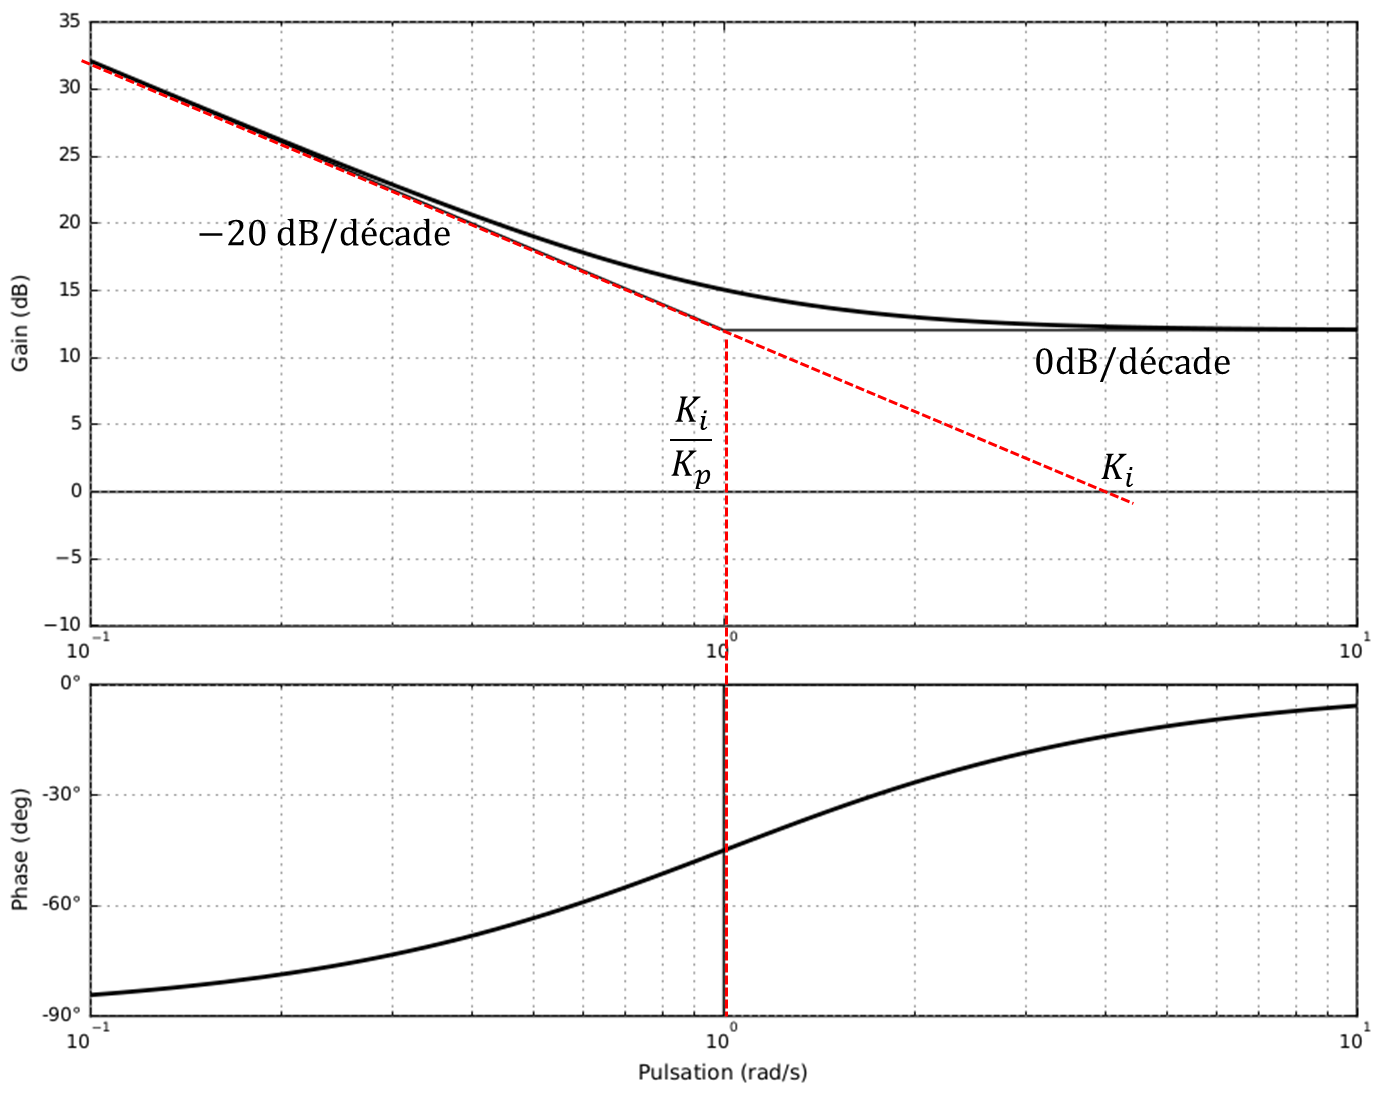
\includegraphics[width=12cm]{63_03_cor}
\end{center}


\else 
\fi


\question{Quelle est l’influence d’un tel correcteur sur la précision et la stabilité ? Justifier.}
\ifprof
Ce correcteur augmente la classe de la FTBO donc augmente la précision. 
Cependant, il réduit la phase. Il faut donc veiller à ce que la pulsation de cassure soit réglée de telle sorte que le système ne soit pas déstabilisé. 
\else 
\fi


\question{Quelle valeur faut-il donner à $\omega_{\SI{0}{dB}}$ pour répondre au critère de rapidité du cahier des charges ?}
\ifprof
D'après la remarque, on a $t_e \omega_{\SI{0}{dB}}=3$ soit $\omega_{\SI{0}{dB}} =3/t_e = \SI{0,075}{rad.s^{-1}}$.
\else 
\fi


\question{Déterminer analytiquement le rapport $T=\dfrac{K_p}{K_i}$ pour obtenir la marge de phase spécifiée dans le cahier des charges.}
\ifprof
Calculons la fonction de transfert en boucle ouverte non corrigée : 
$\indice{F}{BO}=\dfrac{\indice{K}{pom}}{1+T_2 p}\dfrac{\indice{K}{m}}{1+T_1 p} \indice{K}{cap}$.

Le correcteur doit être réglé pour que $\omega_{\SI{0}{dB}} =\SI{0,075}{rad.s^{-1}}$. 

Calculons la marge de phase. 
$\arg\left(\indice{F}{BO}\right)=-\arg\left(1+T_1p\right)-\arg\left(1+T_2p\right) = -\arctan T_1 \omega -\arctan T_2 \omega $
+
On a donc $\arg\left(\indice{F}{BO}(0,075)\right) = -\arctan (10 \times  0,075) -\arctan (5 \times  0,075)=-57\degres$ soit une marge de phase de $-123\degres$.

Pour atteindre une marge de phase de 60\degres, on peut donc baisser la phase de 63\degres.

Calculons $\arg\left(C(j\omega)\right)=-90+\arctan \left(\dfrac{K_p}{K_i}\omega\right)$.

On cherche donc $\dfrac{K_i}{K_p}$ tel que $\arg\left(C(0,075)\right)=-63$
Soit 
$-90+\arctan \left(\dfrac{K_p}{K_i}0,075\right) =-63$
$\Leftrightarrow \arctan \left(\dfrac{K_p}{K_i}0,075\right) =27$
$\Rightarrow  \dfrac{K_p}{K_i}0,075 =0,51$
$\Leftrightarrow  \dfrac{K_p}{K_i}=6,79$.


\else 
\fi


\question{En déduire les valeurs de $K_i$ et $K_p$ qui permettent de régler rapidité et marge de phase.}
\ifprof
Il faut chercher $K_i$ et $K_p$ pour respecter $\omega_{\SI{0}{dB}}$. Recherchons le gain de la boucle ouverte non corrigée pour $\omega_{\SI{0}{dB}}$.

$\indice{G}{dB}\left(\indice{F}{BO}\right)=20\log\left(\indice{K}{pom}\indice{K}{m}\indice{K}{cap}\right)
-20\log\left(\sqrt{1^2+T_1^2\omega^2}\right)-20\log\left(\sqrt{1^2+T_2^2\omega^2}\right)$

On a alors $\indice{G}{dB}\left(\indice{F}{BO}\right)(0,075) = -0,004-1,94-0,57=\SI{2,52}{dB}$.

Il faut donc baisser le gain de \SI{2,52}{dB}
$\indice{G}{dB}\left(C(p)\right) = 20\log K_i -20\log \omega +20\log\left(\sqrt{1+\left(\dfrac{K_p}{K_i}\right)^2\omega^2}\right) $.

On a alors $\indice{G}{dB}\left(C(0,075)\right) = 20\log K_i +22,5+1 = -2,52$ soit $K_i = 10^{-\dfrac{2,52+1+22,5}{20}  } =0,05$.

Par suite, $K_p = 6,79 \times 0,05 = 0,34$.

(\textbf{A vérifier}).

\else 

On donne les diagrammes de Bode en gain et en phase de la fonction de transfert en boucle ouverte corrigée avec le correcteur Proportionnel Intégral déterminé précédemment. On donne sa réponse temporelle avec et sans débit de fuite pour une pression de consigne d’eau de 800 bars.

\fi



\question{La réponse du système est-elle satisfaisante au regard du cahier des charges ? Justifier.}
\ifprof
\begin{center}
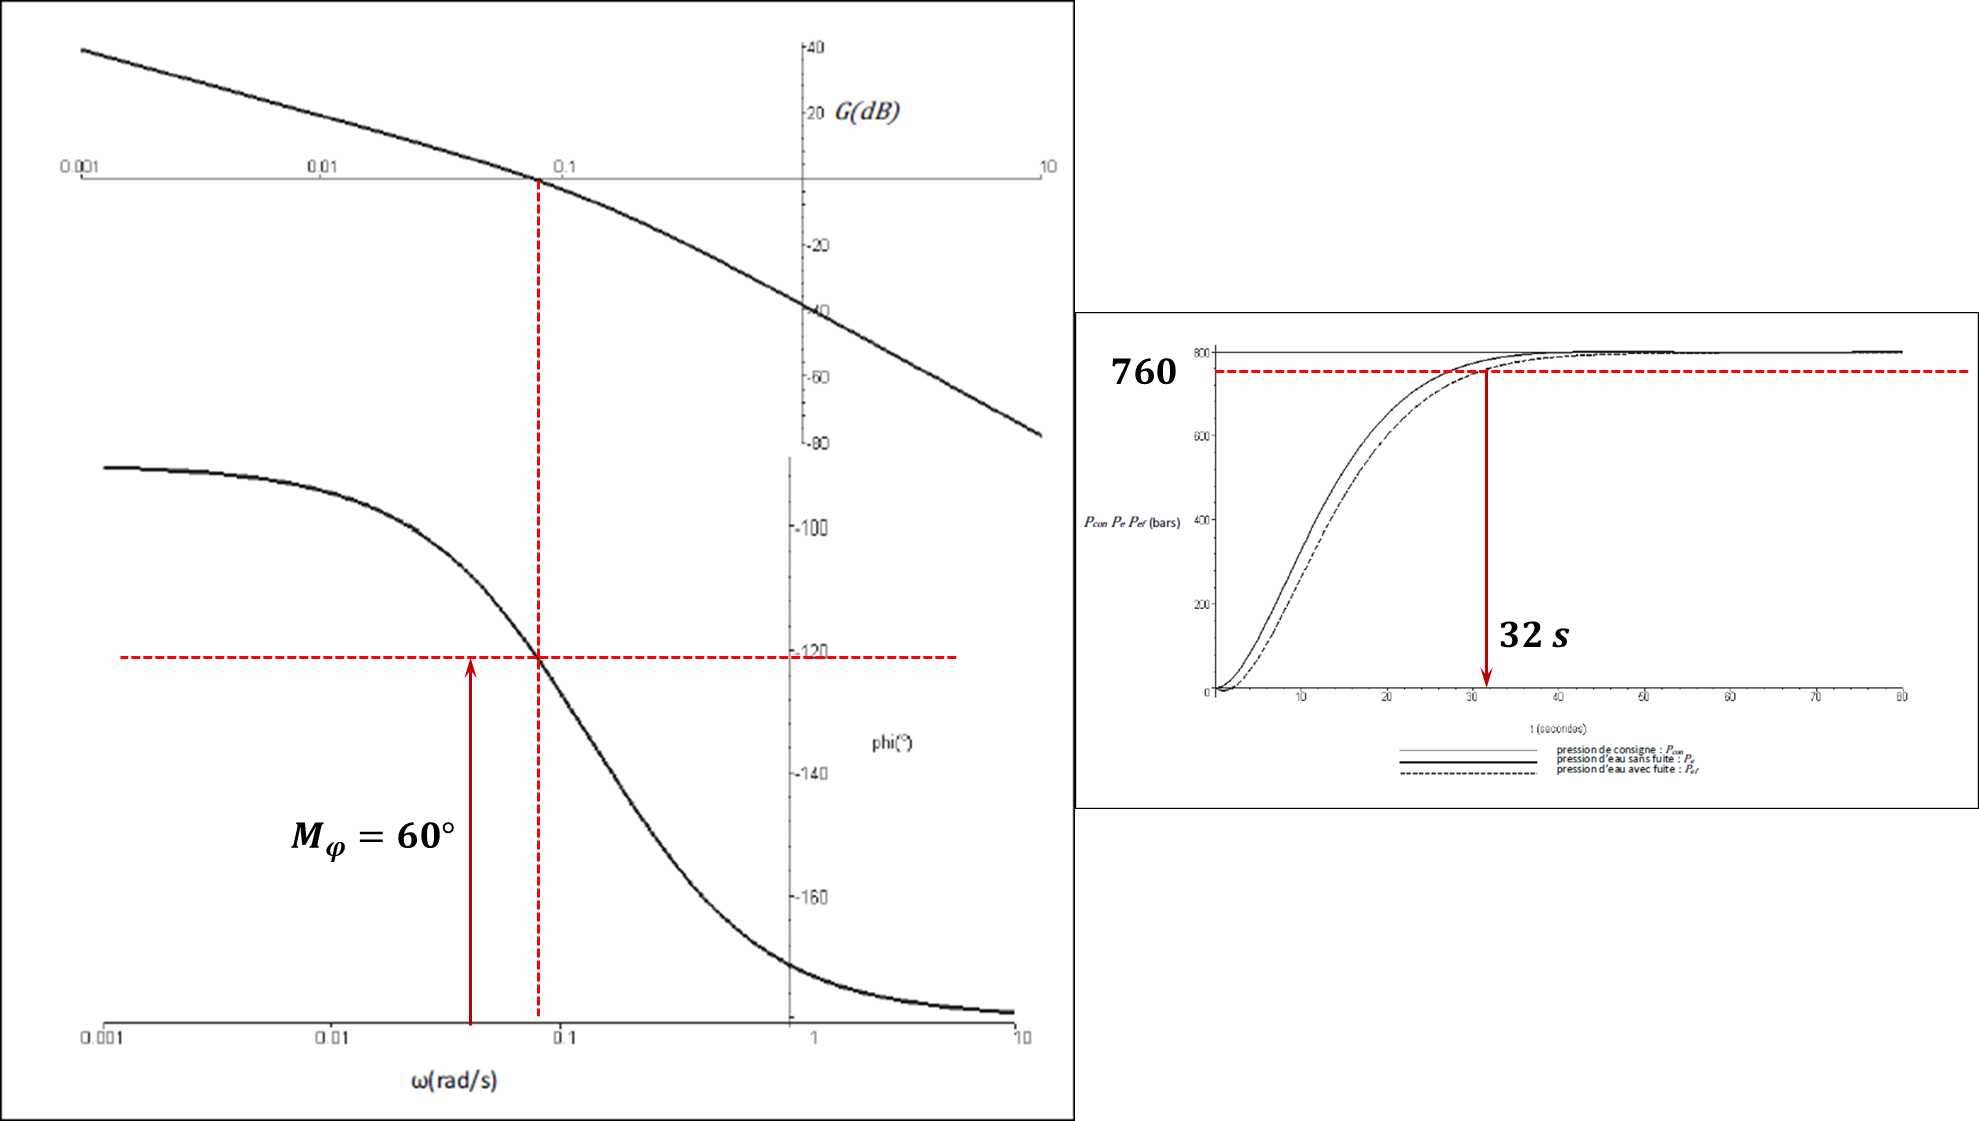
\includegraphics[width=16cm]{63_04_cor}
\end{center}
\begin{itemize}
\item Stabilité : 
\begin{itemize}
\item Marge de phase mesurée :  60\degres \textbf{cdc ok}.
\item Marge de gain mesurée :   infini \textbf{cdc ok}.
\end{itemize}
\item Rapidité : $ t_e = \SI{32}{s} < \SI{40}{s}$ \textbf{cdc ok}.
\item Précision :  écart statique nul \textbf{cdc ok}.
\item Amortissement :  nul \textbf{cdc ok}.
\end{itemize}
\else 
\fi

\ifprof
\else

\begin{center}
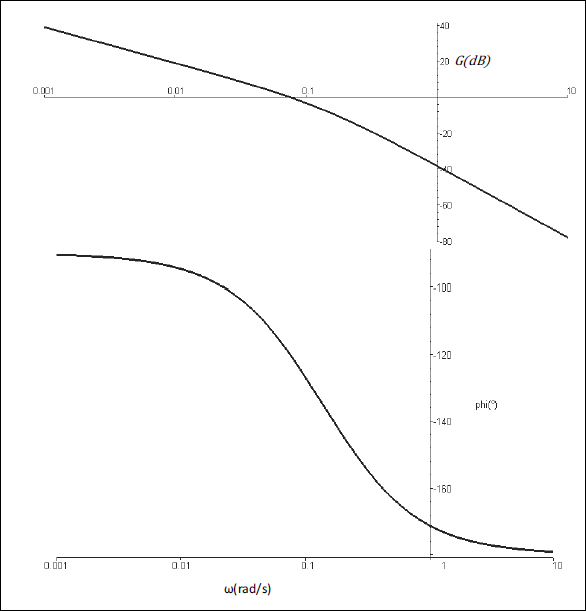
\includegraphics[width=\linewidth]{63_03}
\end{center}


\begin{center}
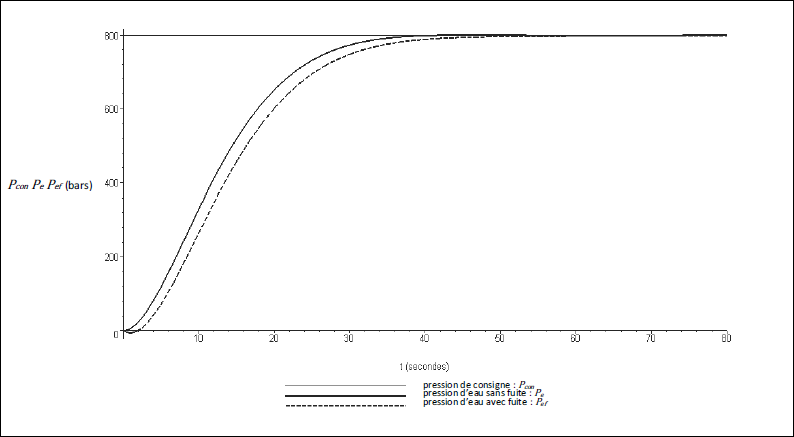
\includegraphics[width=\linewidth]{63_04}
\end{center}
\fi

\ifprof
\else

\noindent\footnotesize
\fbox{\parbox{.9\linewidth}{
Éléments de corrigé : 
\begin{enumerate}
  \item $C(p)= K_i \dfrac{1+p \dfrac{K_p}{K_i}}{p}$.
  \item .
  \item .
  \item $T = 6,79$.
  \item $K_i = 0,05$ et $K_p=0,34$ (à vérifier).
\end{enumerate}}}
\normalsize

\begin{flushright}
\footnotesize{Corrigé  voir \ref{C2:03:stab:63}.}
\end{flushright}%
\fi